\section{Proposed Architecture}
A better zoomable representation of these diagrams can be found in the github repository of this project in /doc/pflichtenheft/pics, where also the xml sources are.
\subsection{Overview}

\hspace{-3cm} 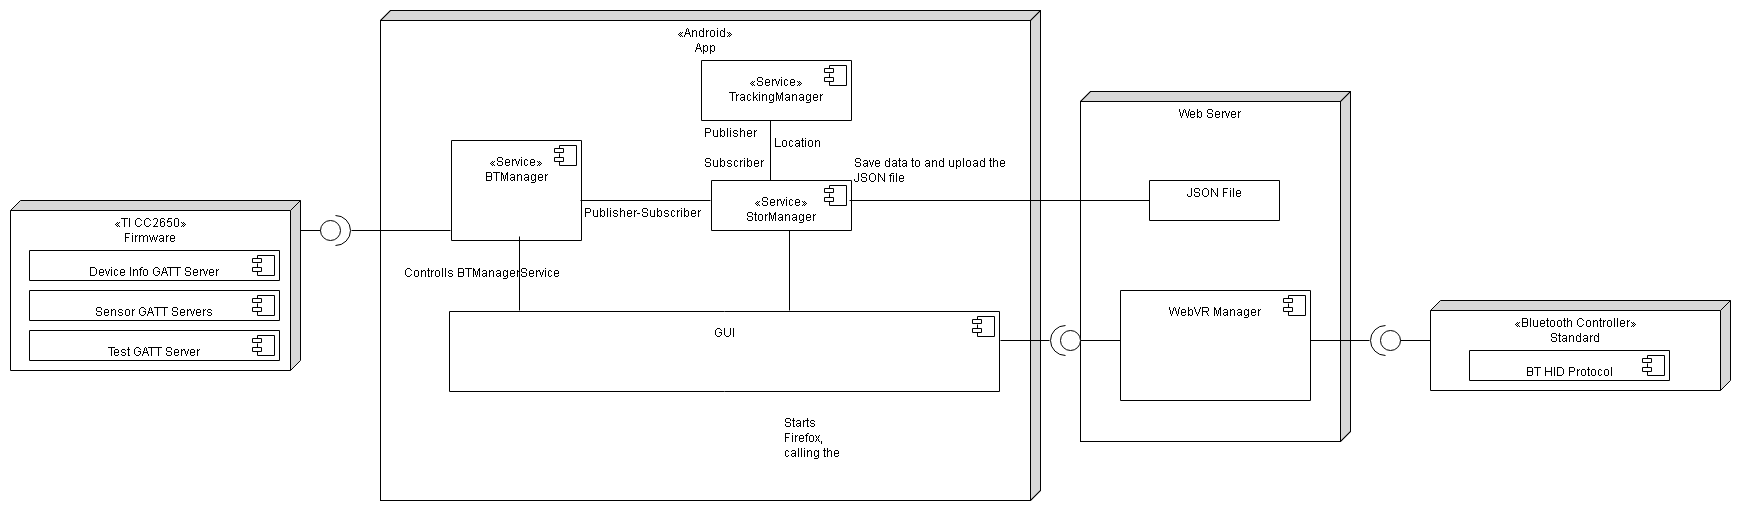
\includegraphics[width=1.4\textwidth]{pics/composite_app.png}


\subsection{Component Decomposition}

\subsubsection{Services}

\begin{itemize}
  \item \textbf{BluetoothManager:} Uses the android.bluetooth and especially the android.bluetooth.le libraries to fetch the sensor data from the sensor device. \\

 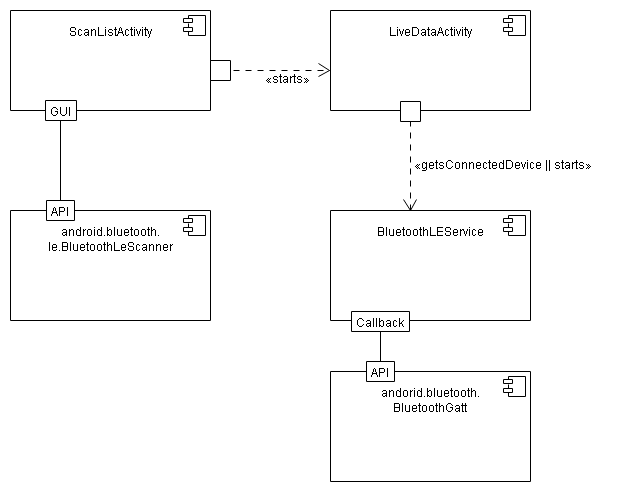
\includegraphics[width=0.8\textwidth]{pics/ble_man.png}

  \item \textbf{TrackingManager:} Handles the tracking of the (current) location where the data are recorded. The current position is determined by GPS and enhanced by the cellphone sensor and wifi data.

 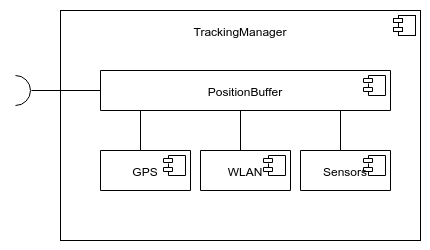
\includegraphics[width=0.8\textwidth]{pics/TrackingManager_Composition.png}

  \item \textbf{StorageManager:} Processes the data provided by the TrackingManager and the BluetoothManager. Uses a JSON file to store data.

 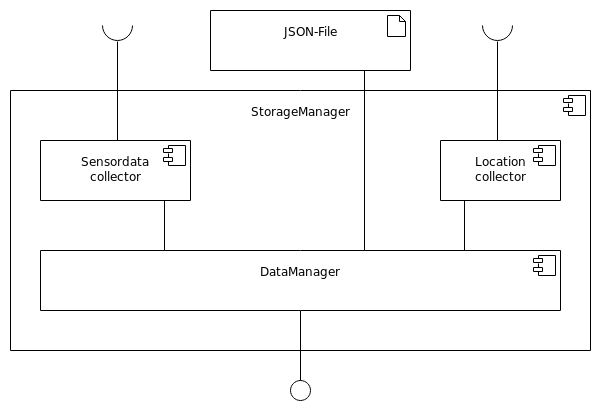
\includegraphics[width=0.8\textwidth]{pics/StorageMgr_Composition.png}

  \item \textbf{WebVRManager:} Handles the display of the virtual reality scene and the given data from the sensor.

 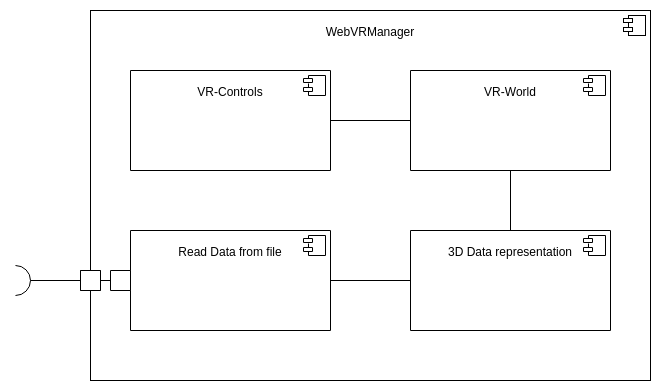
\includegraphics[width=0.8\textwidth]{pics/WebVRManager.png}

\end{itemize}

\subsubsection{GUI}

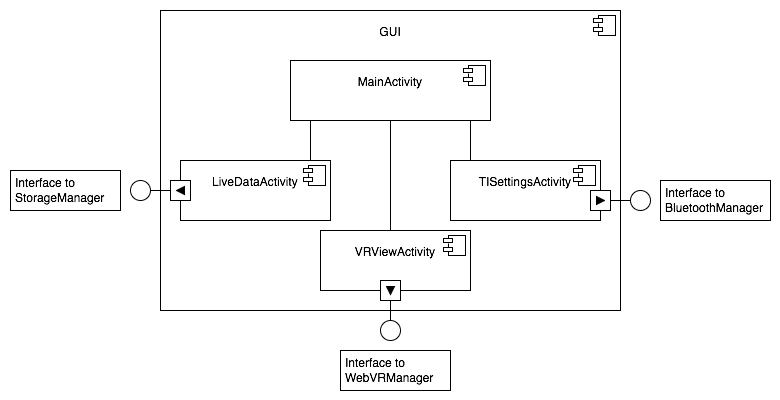
\includegraphics[width=0.8\textwidth]{pics/GUI.png}

\begin{itemize}
  \item \textbf{MainActivity} Provides the main startup screen as the main entry point.
  \item \textbf{VRViewActivity} Shall open a new browser window to display the WebVR webpage.
  \item \textbf{LiveDataActivity} Shall provide a view of the sensor data in human readable form.
  \item \textbf{Settings:} Shall provide a settings screen containing scanning and connecting, connected devices and device settings fragments.
  \begin{itemize}
    \item \textbf{ScanListActivity} shall show the scanning results, delivered by the android.bluetooth.le.BluetoothLeScanner and connect on click on the device.
    \item \textbf{DeviceControlActivity} shall provide propper read and write functions to show and edit the following configuration options of the sensors on the CC2650: Enable/disable the sensor, enable/disable the notifications, disconnect.
  \end{itemize}
\end{itemize}

\subsubsection{Additional Classes}
\begin{itemize}
  \item \textbf{GATT TI CC2650 Service UUIDs}
  \item \textbf{Parser and helper functions for each sensor} because the BLE protocol implemented in the TI CC2650 delivers raw sensor output
\end{itemize}

\subsection{Hardware/ Software mapping}

The app consists of two parts both parts run on the users smart phone, the app will connect to the bluetooth sensor, gather the data and store
it on a web server. The web application will also run on the users smart phone and will be executed in the browser, while the user can start this
browser from the app. The web application will show the scene and display the previously saved data from the sensor in virtual reality.

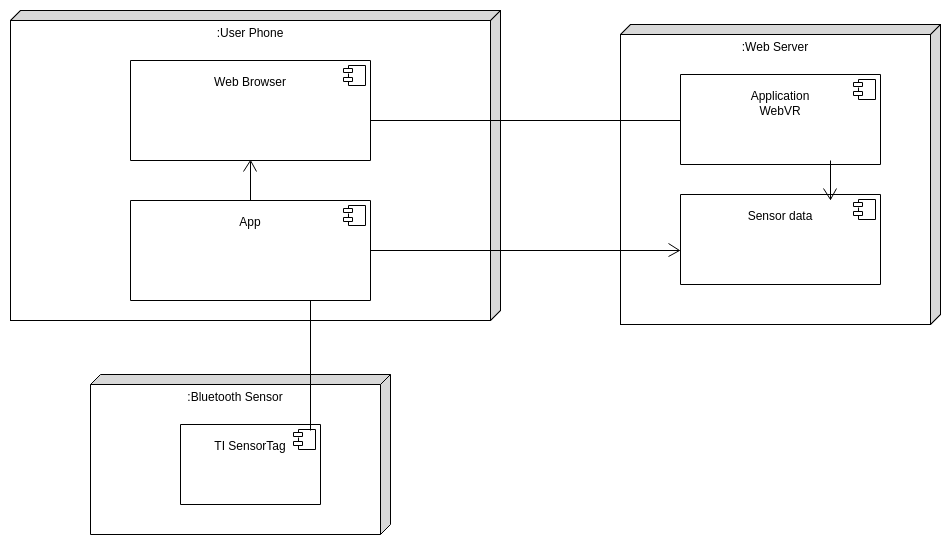
\includegraphics[width=0.8\textwidth]{diagramms/hsMapping.png}

%TO DO ???

%\subsection{Persistent data management}
%TO DO

\subsection{Global software control}
\subsubsection{Startup behavior}
\textbf{User:} The user can start the app by pressing the icon on his screen.
The app will show a startup screen and then transition after a short time into the main menu, from where the user can start the other functions of the app.

\subsubsection{Interfaces}
The \textbf{BluetoothManager} provides a possibility to connect to a sensor and then record
the data. It ensures that a connection is established and that the data are broadcasted via a local BroadcastManager. The first listing below contains the names of the intents and what extra data they contains. The second one lists the interfaces of the ServiceConnection, that's used to bind the service. \\
\begin{lstlisting}
/**
 * @trigger is broadcasted if the Bt.-Adapter of the smartphone
 * connected successfully to the Generic Attribute Profile Server.
 * @data no extra data
 */
public final static String ACTION_GATT_CONNECTED =
        "kn.uni.inf.sensortagvr.ble.ACTION_GATT_CONNECTED";

/**
 * @trigger broadcasted if the Bt.-Adapter of the smartphone
 * disconnected from the Generic Attribute Profile Server.
 * @data no extra data
 */
public final static String ACTION_GATT_DISCONNECTED =
    "kn.uni.inf.sensortagvr.ble:ACTION_GATT_DISCONNECTED";

/**
 * @trigger broadcasted if the services of the connected
 *GATT Server are discovered.
 * @data no extra data
 */
public final static String ACTION_GATT_SERVICES_DISCOVERED =
    "kn.uni.inf.sensortagvr.ble:ACTION_GATT_SERVICES_DISCOVERED";

/**
 * @trigger broadcasted if a characteristic was read, if a
 * characteristic value changed (notification) or if
 *the RSSI is read.
 * @data EXTRA_DATA, float[3]
 * @data EXTRA_SENSOR, Sensor or "RSSI"
 *
 * Sensor is an enum that defines the following fields: UUID service, UUID data, UUID config, byte enablecode
 * There is a getDataFromUUID() method, that returns the last read value for this UUID
 * !This is not the measured but a safed value!; measurement is done via service connection/notifications
 */
public final static String ACTION_DATA_AVAILABLE =
    "kn.uni.inf.sensortagvr.ble.ACTION_DATA_AVAILABLE";

/**
* Contains an element of the Sensor enum or the string "RSSI"
* (not in that enum because it has no UUIDs at all)
*/
public final static String EXTRA_SENSOR =
    "kn.uni.inf.sensortagvr.ble.EXTRA_SENSOR";

/**
* Contains converted raw data stored in a float array with 3 places
*/
public final static String EXTRA_DATA =
        "kn.uni.inf.sensortagvr.ble.EXTRA_DATA";
\end{lstlisting}
\begin{lstlisting}
ServiceConnection
	void onServiceConnect(ComponentName c, IBinder b);
	void onServiceDisconnected(ComponentName c);
ServiceMethods
	boolean connect(String address);
	void disconnect();
	boolean enableSensor(Sensor s);
	boolean disableSensor(Sensor s);
	void readCharacteristic(BluetoothGattCharacteristic c);
	void setCharacteristicNotification(BluetoothGattCharacteristic
	 c, boolean b);
	void broadcastCharacteristic(BluetoothGattCharacteristic c);
	void writeConfigCharacteristic(BluetoothGattCharacteristic
	 c, byte b);
	List<BluetoothGattService> getSupportedGattServices();
Sensor enum
	UUID getService(Sensor s)
	UUID getData(Sensor s)
	UUID getConfig(Sensor s)
	Sensor getSensorFromUUID(UUID u);
	byte getEnableSensorCode(Sensor s)
	float[] convert(byte b);
\end{lstlisting}

\noindent The \textbf{StorageManager} provides a possibility to store the data from the sensor together with the current position.
It also can store the data in a .json file and upload them to a webserver.

\begin{lstlisting}
InterfaceStorageManager {
  public void setSensor(integer internalSensorID){
    activeSensor = internalSensorID;
  }
  //tells the storage manager to get data from the active sensor and
  //the tracing manager, mark them with a timestamp and store the data
  //in a DataSet.
  public void measureNow(){
  }
  //get the latest measured DataSet of the active sensor
  public DataSet getLiveData() {
    return DataSet;
  }
  //get a DataSet which contains data of the activeSensor and position
  //at the specified time. If no data was stored at that time, an empty
  //DataSet will be returned.
  public DataSet getDataFrom(int time) {
    return DataSet;
  }
  //get multiple DataSets which contain all measured Data from the
  //active Sensor between 'time' and now.
  public DataSet[] getDataSince(int time) {
    return DataSet[];
  }
  // Upload the data set to a webserver
  // a .json file from time till now.
  public void uploadData(int time) {
    //upload the data to a server so webvr can later use it.
  }
}
\end{lstlisting}


The \textbf{TrackingManager} gets the current location of the smartphone and provides it to the rest of
the App.

\begin{lstlisting}
Interface TrackingManager {
  //get the current location of the device
  public Location p getCurrentPosition() {
    ensures iff lockCustomPos
      p == customPos;
      else
        p == currentPosition;
  }
}
\end{lstlisting}


The \textbf{VRBox} gets the data from a webserver and loads it into the VR-World.

\begin{lstlisting}
Interface WebVR {
  //Load the data from the webserver to display in VR.
  //The data will be a .json file which will be parsed
  // by in javascript by the web page.
  function loadData(file){
  }
}
\end{lstlisting}

\subsubsection{Sequences}

\begin{description}
	\item[1) Start VR view:] When the user clicks a button to start the VR view, a web browser is opened via an intent.  \\
	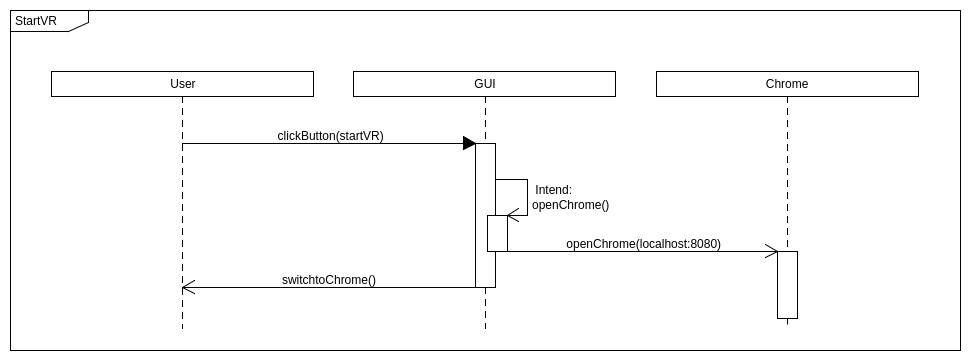
\includegraphics[width=0.8\textwidth]{diagramms/startVR.png}

	\item[2) Switch to stereoscopic 3D: ] When the user enters the VR view, he can choose to switch the view and thereby switch to a stereoscopic view or switch back to non-stereoscopic view, respectively. \\
	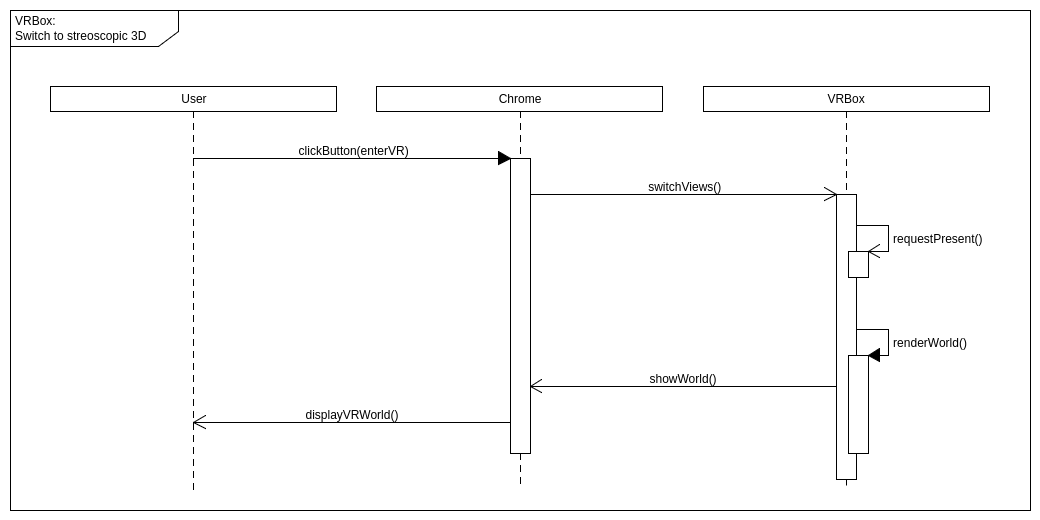
\includegraphics[width=0.8\textwidth]{diagramms/stereo.png}

	\item[3) Switch data visualization: ] When the user opens the web site with the VR view, he  can switch the visualization. The first view is a plane composed from
  the location tracking together with the data from the sensor, the second visualization is a representation of the locations as dots
  and the data as numbers hovering over these dots.  \\
	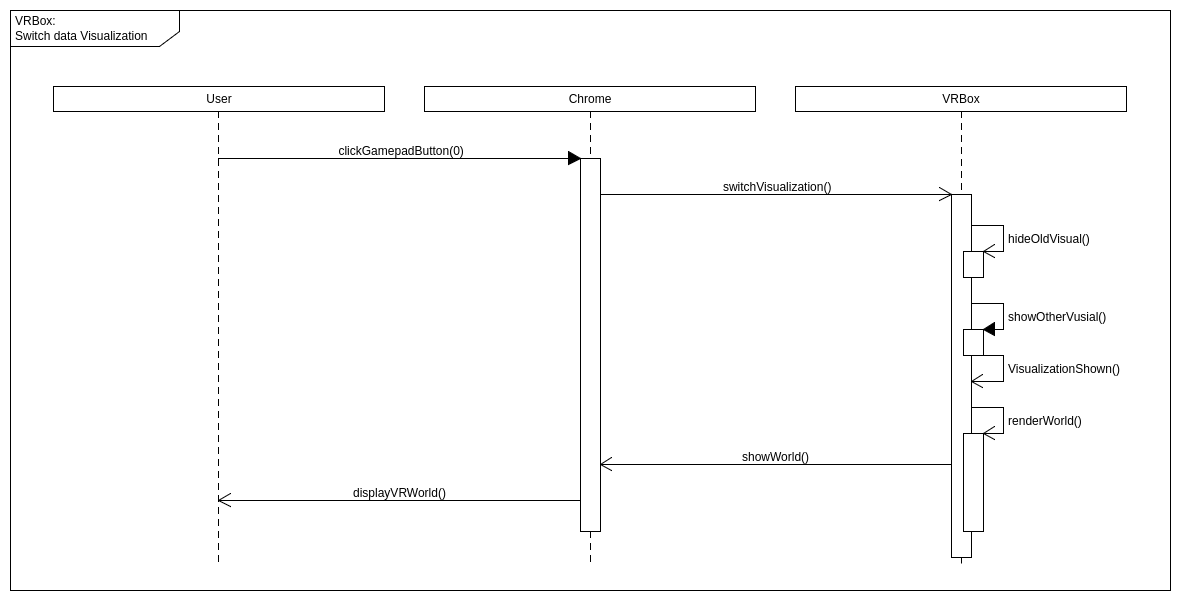
\includegraphics[width=0.8\textwidth]{diagramms/switchVisual.png}

	\item[4) Scan and Connect:] Scan for Bluetooth low energy devices and connect to one of them by clicking on the correct result ("TI CC2650").
	After beeing connected one can edit the configuration of the sensors on the CC2650: \\dis-/enable a sensor, (de-)activate the notifications for a measurement characteristic, read values, disconnect from the device. After that the user may start a new data scan record or start the VR View.\\
	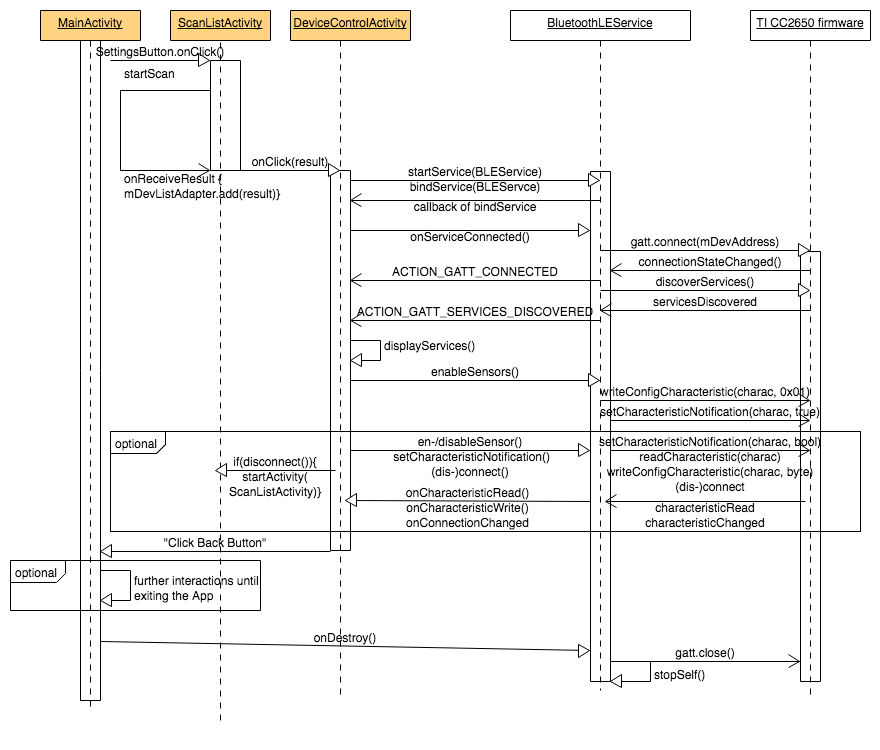
\includegraphics[width=0.8\textwidth]{diagramms/bleseq.png}

	\item[6) Record new data set: ] When the user clicks the button to record a new data set, the StorageManager will provide the data and get the repective location from the TrackingManager to calibrate the initial location for the recording session. \\
	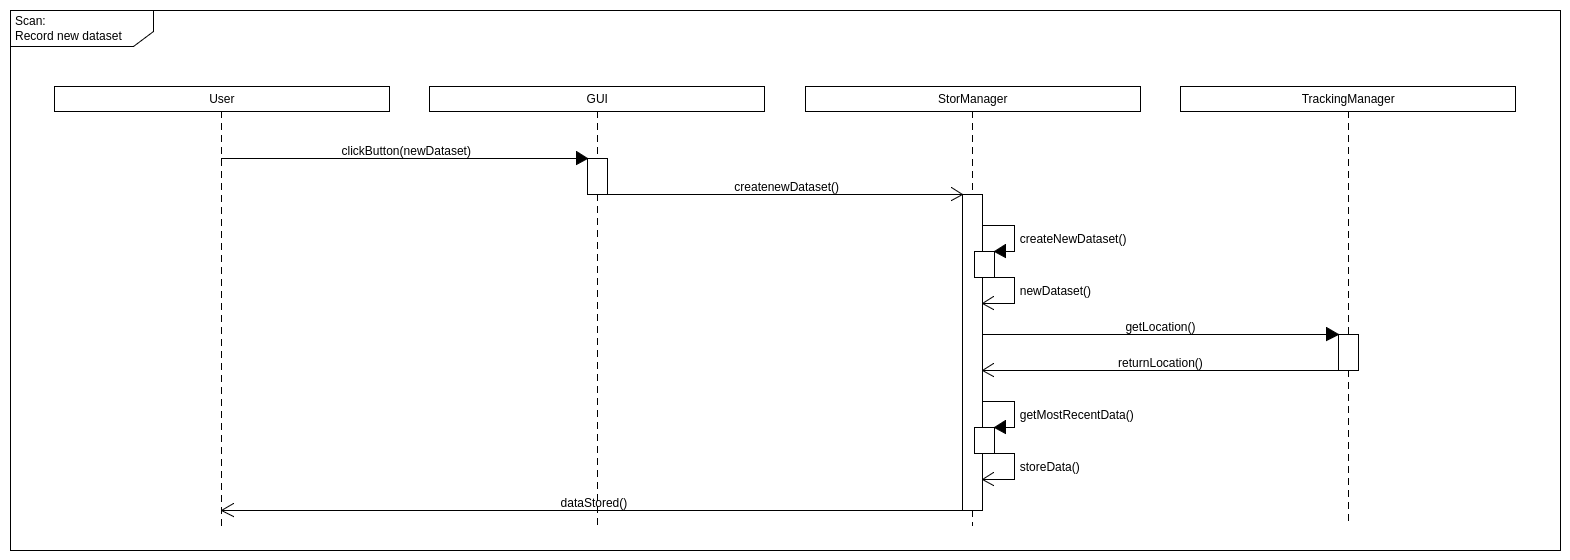
\includegraphics[width=0.8\textwidth]{diagramms/newDataset.png}

	\item[7) Record data point: ] When the user clicks the button to record new data, the StorageManager will provide the data and get the repective location from the TrackingManager.\\
	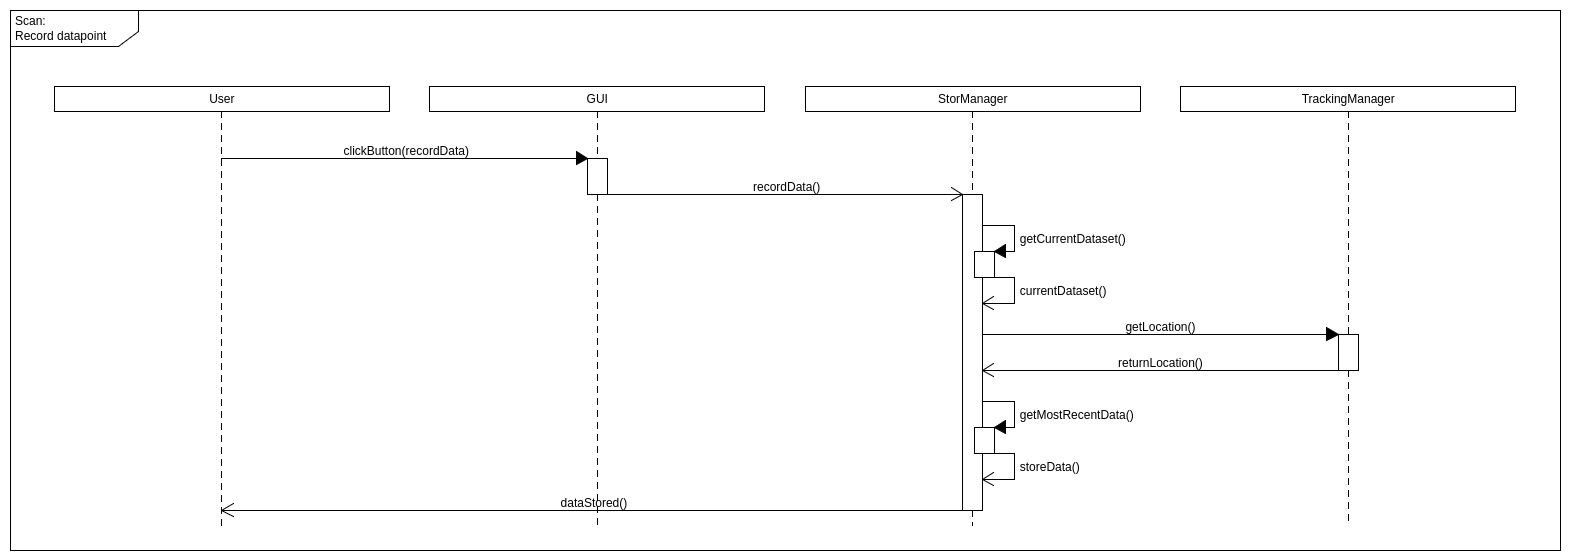
\includegraphics[width=0.8\textwidth]{diagramms/recordDatapoint.png}



\end{description}
